\section{Computing Rectification Functions}\label{sec:rfunc}

% The {\it multi-fix rectification theorem} determines whether there 
% exists a set of polynomial functions $U = (u_1,\dots,u_m)$  
% such that substituting every patch function $u_i$ as the $tail$ 
% at its respective target $w_i$, for $i = 1,\dots,m$, makes $C$ 
% functionally equivalent to $\spec$. 
% We formulate the computation of rectification function by extending 
% the decision procedure to a quantification 

For a given set of targets $W$, due 
to the presence of don't cares (DC), there may exist more 
than one set $U$ of rectification functions which will rectify the circuit.
In this section, we describe the notion of DC 
in the MFR setup which can be exploited for the simplification
of rectification patches.
Exploring all the DC conditions for $m$ targets might be computationally infeasible; we
present two different approaches to overcome this. First,
we present an approach to compute an on- and off-set for each rectification function by 
heuristically resolving all the DC conditions.
Following this, we present an approach to 
explore and compute a subset of the DC conditions, along with 
on- and off-sets, for each rectification function.

% In this section, we describe the notion of DC 
% in the MFR setup which can be exploited for further simplification
% of rectification patches.
% % for synthesis of efficient rectification patches.
% However, it is infeasible to explore and analyze all the possible DC-sets. 
% To overcome this complexity, we first present a 
% greedy heuristic which computes a rectification function 
% set $U$ by eliminating all the DC conditions.
% % We first present a greedy approach which quickly computes an on- and off-set for each rectification patch. 
% Following this, we present an approach to explore and compute a subset of 
% the DC conditions, along with on- and off-sets, for the given targets.

% \vspace{-0.2in}
% , such that substituting the patches
% into the polynomial set $F$ $(f_{w_1}:w_1+u_1,\dots,f_{w_m}:w_m+u_m)$ 
% rectifies the circuit.

% This involves computing a {\bf reduced \Grobner basis} for the polynomial $rem_l$ and then 
%  From the ideal $J$, a polynomial $U$ can be computed
% using Lagrange interpolation,
% which evaluates to 0 on $V(J)$ and 1 everywhere else $i.e.$ $V(U)=V(J)$. 
% % Due to the formulation of Lagrange interpolation, 
% The polynomial
% $U$ has variables in the set $\xpi$, and coefficients in $\{0,1\}$; $U \in \F_2[\xpi]$.
% Therefore, $U$ always evaluates to either 0 or 1 for any value of
% $\xpi$ variables. 

% After computing $\uc$, we can patch the circuit
% with the polynomial $f_i: x_i + \uc$.

% \subsection{Background}
% A \Grobner basis computed using Buchberger's algorithm is not a canonical
% representation of an ideal in itself. To obtain the canonical representation of
% an ideal, we need to compute a {\bf reduced \Grobner basis}. A reduced \Grobner basis
% is computed by first computing a minimal \Grobner basis, and then reducing it.

% \begin{Definition}\label{def:minigb}
% A {\bf minimal Gr\"obner basis} $G=\{g_1,\dots,g_t\}$ for a polynomial ideal $I$ is a \Grobner basis for $I$ such that
%     \begin{itemize}
%         \item $lc(g_{i})=1,\forall g_{i}\in G$
%         \item $\forall g_{i} \in G$,  $lt(g_{i}) \notin \langle lt(G-\{g_{i}\})\rangle$
%     \end{itemize}
% \end{Definition}
% A {\bf minimal} \Grobner basis is a \Grobner basis such that all polynomials
% have a coefficient of $1$ and no leading term of any element in $G$ divides 
% another in $G$.
% Given a \Grobner basis $G$, a minimal \Grobner basis can be
% computed as follows:
% \begin{enumerate}
% \item Make every $g_i \in G$ monic, i.e $g_i=g_i/lc(g_i)$
% \item For $g_i, g_j \in G$ where $i\neq j$, remove $g_i$ from $G$ if $lt(g_i)\mid lt(g_j)$, i.e. remove every polynomial in $G$ whose leading term is divisible by the leading term of some other polynomial in $G$.
% \end{enumerate}

% Then $G$ is minimal $w.r.t.$ number of elements. 
% A minimal Gr\"obner basis can then be further reduced.
% \begin{Definition}
%     A {\bf reduced Gr\"obner basis} for a polynomial ideal $I$ is a Gr\"obner basis $G=\{g_{1},\dots,g_{t}\}$ such that:
%     \begin{itemize}
%         \item $lc(g_{i})=1,\forall g_{i}\in G$
%         \item $\forall g_{i} \in G$, no monomial of $g_{i}$ lies in $\langle lt(G-\{g_{i}\})\rangle$
%     \end{itemize}
% \end{Definition}
% $G$ is a reduced Gr\"obner basis when no monomial of any element in $G$ is
% divisible by the leading term of another element. 

% \subsection{Computing Rectification Patches}
\subsection{Greedy Approach for MFR}\label{comp:GFC}

To illustrate the greedy approach, consider the case with $m = 2$, where $W_c = \{(0,0), (0,1), (1,0), (1,1)\}$, and we must compute rectification functions $u_1$ and $u_2$. For brevity, let $V_{W_c[i]} = V(rem_i)$, for $1 \leq i \leq 2^m$; in this case, $V_{(0,0)} = V(rem_1)$, $V_{(0,1)} = V(rem_2)$, and so on.

Recall that $V_{(0,0)}$ comprises the set of points where the $\impl$ and $\spec$ evaluate the same for the corresponding assignments $(0,0)$ to the targets. This implies that at these points, the rectification functions $u_1$ and $u_2$ should evaluate to $0$. Table~\ref{tab:tar_assign} shows the required evaluations of $u_1$ and $u_2$ for the points in each variety, following the same reasoning. The on-set of the rectification function for a target corresponds to the union of the varieties (sets) where the function evaluates to $1$, and the off-set corresponds to the union of the varieties (sets) where the function evaluates to $0$. In this case,
the on-set of $u_1$ consists of the set of points in $V_{(1,0)} \cup V_{(1,1)}$, and the off-set of $u_1$ consists of the set of points in $V_{(0,0)} \cup V_{(0,1)}$. Similarly, the on-set and off-set of $u_2$ consists of the points in $V_{(0,1)} \cup V_{(1,1)}$ and $V_{(0,0)} \cup V_{(1,0)}$, respectively. The functions $u_1$ and $u_2$ could be
synthesized using these on- and off-sets.

\begin{table}[hbt!]
  \centering
  \caption{Function evaluations }\label{tab:tar_assign}
  \begin{tabular}
    {!{\vrule width 1pt} c !{\vrule width 1pt} c | c !{\vrule width 1pt}}\noalign{\hrule height 1pt}
    {\textit Variety} & {$u_1$} & {$u_2$} \\ \noalign{\hrule height 1pt}
    $V_{(0,0)}$             & 0       & 0       \\ \hline
    $V_{(0,1)}$             & 0       & 1       \\ \hline
    $V_{(1,0)}$             & 1       & 0       \\ \hline
    $V_{(1,1)}$             & 1       & 1       \\ \noalign{\hrule height 1pt}
  \end{tabular}
\end{table}
    
However, the above argument is only correct when $V_{(0,0)}, V_{(0,1)}, $ $ V_{(1,0)}, V_{(1,1)}$ are pairwise disjoint, which may not be true in practice. For example, for a point contained in $V_{(0,0)} \cap V_{(0,1)}$, $(u_1,u_2)$ must evaluate either to $(0,0)$, or to $(0,1)$ in order for the $\impl$ to evaluate to the same value as the $\spec$; this point would be in both the on- and off-set of $u_2$ in the method previously described. A decision procedure is necessary to determine the evaluation of $(u_1,u_2)$ at these intersections. 
We present a greedy approach which resolves such ambiguities by imposing an order on the sets.
An example of our greedy approach to evaluate $(u_1,u_2)$ for an order $V_{(0,0)} > V_{(0,1)} > V_{(1,0)} > V_{(1,1)}$ is as follows:

% One complication arises from the fact that the intersections of these varieties might not be empty.  
% % These points are in the off-set of $u_1$, however, they are in the on-set and off-set of $u_2$
% Therefore, $u_1$ must evaluate to $0$, but $u_2$ may evaluate either to $0$ or to $1$; the choice will change the resulting patch function. For points in any intersection between any of the sets $V_{(0,0)}, V_{(0,1)}, V_{(1,0)}, V_{(1,1)}$, a similar choice must be made, resulting in an exponential number of potential distinct rectification functions.  A simple approach to overcome this complexity and construct a rectification function for each target is as follows: 

First, we place all the points from $V_{(0,0)}$ into the off-sets of $(u_1, u_2)$. Next, we place all the points from $V_{(0,1)} \setminus V_{(0,0)}$ into the off-set of $u_1$ and the on-set of $u_2$. We perform the set difference to avoid placing the points in $V_{(0,0)} \cap V_{(0,1)}$ into both the on-set and off-set of $u_2$. Next, we place all the points from $V_{(1,0)} \setminus (V_{(0,0)} \cup V_{(0,1)})$ into the on-set of $u_1$, and the off-set of $u_2$. Finally, we place the remaining points from $V_{(1,1)} \setminus (V_{(0,0)} \cup V_{(0,1)} \cup V_{(1,0)})$ into the on-set of $(u_1, u_2)$.
% \begin{figure}[hbt]
%     \begin{center}
%     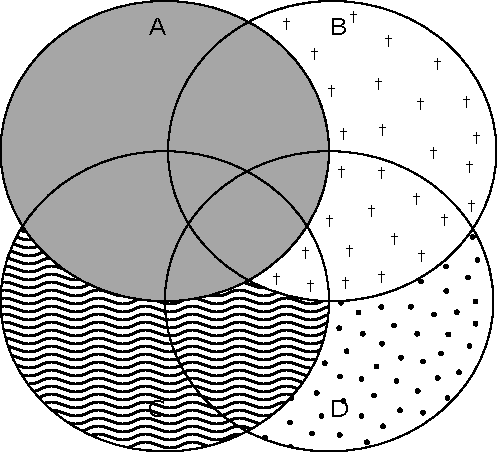
\includegraphics[scale = 0.31]{simple_rect_func1.pdf}
%     \end{center}
%     \caption{{\footnotesize  
%       Rectification function computation
%       illustrated for two targets}}  
%     \label{fig:simp_rec_func}
%     % \vspace{-0.25in}
% \end{figure}
% Thus, for a target $u_i$, the on-set corresponds to the union of the sets where $u_i$ evaluates to $0$, 
% and the off-set corresponds to the union of the sets where $u_i$ evaluates to $1$. 
The resulting on- and off-sets for $u_1$ and $u_2$ are shown below.

\begin{small}
\begin{align*}
  \begin{split}
    V(u_{1_{on}})&= (V_{(1,1)} \setminus (V_{(0,0)} \cup V_{(0,1)} \cup V_{(1,0)})) \cup (V_{(1,0)} \setminus (V_{(0,0)} \cup V_{(0,1)}))\\
    V(u_{1_{off}}) &= (V_{(0,0)}) \cup (V_{(0,1)} \setminus V_{(0,0)}) \\
    V(u_{2_{on}})&= (V_{(0,1)} \setminus V_{(0,0)}) \cup (V_{(1,1)} \setminus (V_{(0,0)} \cup V_{(0,1)} \cup V_{(1,0)}))\\
    V(u_{2_{off}}) &= (V_{(0,0)}) \cup (V_{(1,0)} \setminus (V_{(0,0)} \cup V_{(0,1)}))
  \end{split}
\end{align*}
\end{small}

This approach with the given order greedily places points into the off-sets of the rectification functions $(u_1, u_2)$ where possible, and only places points into the on-sets of the rectification functions when necessary. 
Subject to the given order, the on-sets of the rectification functions are thus minimized. For the experiments in this paper, we always use the order
$V_{W_c[i]} > V_{W_c[j]}$ for $i < j$, as in the above example, though any order would yield valid rectification functions. 

Generalizing our greedy approach for $m$ targets, we first
construct the following composite sets (varieties):
\begin{equation}
  \label{eqn:composite_greedy}
  S_l=
  \begin{cases}
    V_{W_c[1]},                                                & \text{if}\ l=1   \\
    V_{W_c[l]} \setminus (\bigcup\limits_{j=1}^{l-1}V_{W_c[j]}), & 2\leq l \leq 2^m
  \end{cases}
\end{equation}

The resulting on-set and off-set functions for each target $i$, where $1 \leq i \leq m$ are: 
\begin{align}
  \label{eqn:ui_on_off}
  \begin{split}
  V(u_{i_{on}}) &= \bigcup S_l,~\forall l~|~W_c[l][i]=1 \\
  V(u_{i_{off}}) &= \bigcup S_l,~\forall l~|~W_c[l][i]=0
  \end{split}
\end{align}

% Vikas, can you help me write this paragraph? Something about how 
% 1. this gives us the varieties of u_i, but we can't find those directly, so instead we use
% the product of rem_l's and colon ideals to find the set unions and differences and end up with a polynomial
% whose variety is V(u_ion), V(u_ioff). Or something like that. 



% Since the approach resolves all the DC conditions instantly, the computed composite sets $S_l$ 
% are pairwise disjoint. As a result, the on- and off-sets for each target are 
% complements of each other. Hence, one can 
% use either $u_{i_{on}}$ or the complement of $u_{i_{off}}$ for patch function computation.

\subsection{Don't Care Conditions for MFR}\label{comp:DFC1}

% is agnostic to the synthesis cost of $\impl$
% However, we will introduce the notion of word-level don't cares 
% in the MFR setup, which can be further leveraged towards computing a desired solution.
% We want to select a rectification function which has the least synthesis cost 
% (in the number of literals or in the number of AND-XOR operations etc.). 

% Although the greedy approach yields a correct rectification function, it does not compute any Don't Care (DC) conditions, but instead heuristically assigns points to the off-set when possible at the intersections of varieties. 
% DC conditions can be exploited to synthesize efficient patch functions. In this section, we explore the sets of points where DC conditions appear and propose an approach to systematically compute a subset of these DC points for each target.

% For a given target $W$, due to the presence of Don't care (DC), there may exist more 
% than one rectification function ($U$) which will rectify the circuit.
% The choice of these rectification functions can have significant synthesis consequences.
% As shown above, the simple approach presented on computing a rectification 
% function completely eliminates these DC conditions.
% Exploring the complete DC sets for simplification of a rectification function is
% a logic optimization problem and is beyond the scope of this paper.
% However, we will describe and show the existence of DC sets 
% in the MFR setup which can be utilized to converge towards a desired solution.
% , we will introduce the notion of word-level don't cares in the MFR setup.

% \subsubsection{Strong and Conditional Don't Care Conditions}

% We define two distinct types of DC points for circuits with multiple rectification targets: strong don't care ($DC_{st}$) points and conditional don't care ($DC_{cond}$) points. Strong don't care points for a target are defined as the points where the $\impl$ and $\spec$ match when the target evaluates either to $0$ or to $1$ at those points, independent of the evaluations of other targets at those points. By contrast, conditional don't care points for a target are the points where the $\impl$ and $\spec$ match when the target evaluates either to $0$ or to $1$, but where the choice is conditioned on the evaluations of other targets at those points.

% An intersection of varieties contain DC points for a set of rectification functions $u_i, \dots, u_j$ if 1. Every binary combination of evaluations of $u_i, \dots, u_j$ results in $C$ matching the $\spec$, where 2. The remaining rectification functions evaluate either to $1$ or to $0$ for every combination of evaluations of $u_i, \dots, u_j$. 

% For example $V_{(0,0,0)} \cap V_{(0,0,1)} \cap V_{(0,1,0)} \cap V_{(0,1,1)}$ contains DC points for u_2, and u_3, but 
% $V_{(0,0,0)} \cap V_{(0,0,1)} \cap V_{(0,1,0)} \cap V_{(1,1,1)}$ doesn't - it violates #2.
%

Let $U_d \subseteq U$ denote a subset of the target rectification functions. 
We are interested in the DC conditions which arise for these functions at 
points where they may evaluate to any value, for some fixed 
evaluation of the remaining functions in the set $\{U \setminus U_d\}$. 
% Such points exist only at the intersections of varieties.
For example, consider a point in $V_{(0,0)} \cap V_{(0,1)}$ for 
a circuit with two targets. As discussed previously, $u_1$ must evaluate to $0$ at 
this point, but $U_d = \{u_2\}$ may evaluate either to $0$ or to $1$,
so this is a $DC$ point for $u_2$. 


% We will continue with the illustration of $m=2$ with $U=\{u_1,u_2\}$, 
% and let $U_d=\{u_2\}$. The don't care conditions for $u_2$ are the points 
%  Continuing with the $m=2$ 
% illustration, the entire DC condition evaluations for the functions $(u_1,u_2)$ are 
% given as $DC = \{(0,d),(d,0),(d,1),(1,d),(d,d)\}$. Here,
% $d \in \{0,1\}$ denotes a don't care evaluation.
% Not really sure how to talk about these intersections....
Not every intersection of varieties yields $DC$ points 
which follow the conditions described above. 
Consider a point in $V_{(0,0)} \cap V_{(1,1)}$. Here, $(u_1, u_2)$ 
must evaluate either to $(0,0)$ or to $(1,1)$. If this point were 
assigned to the $DC$ set of $u_2$, for example, the $\spec$ and $\impl$ 
would only evaluate the same if $u_1$ evaluated to the same value as $u_2$.  
Thus, $u_1$ would become a function of $u_2$ at this point. This point 
cannot be placed into the on-set, off-set, or DC-set of $u_1$ before $u_2$ 
is evaluated. To avoid inter-dependencies between the rectification functions, we do not classify 
points in such intersections as $DC$ points. We rely on our greedy heuristic to 
evaluate these points. 
% In contrast, in the previous 
% case, $u_1 = 0$ and $u_2 = DC$ for a point in $V_{(0,0)} \cap V_{(0,1)}$. 

% Instead, we can use a heuristic to make a decision to place 
% points in this intersection into the off-set or on-set of both $u_1$ and $u_2$. 
% These constitute $DC_{cond}$ points for both targets because the targets individually may evaluate either to $0$ or to $1$, with the condition that they evaluate to the same value as the other target. 

% Further, some intersections might involve more than two varieties. The intersection 
% $V_{(0,0)} \cap V_{(0,1)} \cap V_{(1,0)} \cap V_{(1,1)}$ constitutes a $DC$ 
% set for both $u_1$ and $u_2$ because at this intersection, every combination 
% of evaluations $(0,0), (0,1), (1,0), (1,1)$ results in the $\spec$ and $\impl$ agreeing. 

Finally, consider a point in $V_{(0,0)} \cap V_{(0,1)} \cap V_{(1,0)}$. 
This point cannot be a DC point for both targets simultaneously 
since the evaluation $(1,1)$ here will result in an incorrect rectification function. 
However, because $V_{(0,0)} \cap V_{(0,1)} \cap V_{(1,0)} \subset V_{(0,0)} \cap V_{(0,1)}$, 
we could treat this point as a $DC$ point for $u_2$ and evaluate $u_1$ to $0$. 
Alternatively, because $V_{(0,0)} \cap V_{(0,1)} \cap V_{(1,0)} \subset V_{(0,0)} \cap V_{(1,0)}$, 
we could treat this point as a $DC$ point for $u_1$ and evaluate $u_2$ to $0$.
Thus, we have a choice to place this point in the $DC$-set of either targets, but not both. 

% In the next section we describe a heuristic to make decisions for points in intersections such as these.

% is not an $DC_{st}$ set for $u_1$ or $u_2$  Instead, this intersection represents a set of $DC_{cond}$ points for both targets because each target individually may evaluate to $0$ or to $1$, with the condition that both targets may not evaluate to $1$. However, because $V_{(0,0)} \cap V_{(0,1)} \cap V_{(1,0)} \subset V_{(0,0)} \cap V_{(0,1)}$, we can treat these points as $DC_{st}$ points for $u_2$ and evaluate $u_1$ to $0$. Alternatively, because $V_{(0,0)} \cap V_{(0,1)} \cap V_{(1,0)} \subset V_{(0,0)} \cap V_{(1,0)}$, we could treat these points as $DC_{st}$ points for $u_1$ and evaluate $u_2$ to $0$. An intersection with $DC_{cond}$ points may or may not be contained in an intersection with $DC_{st}$ points. 

Finding every intersection containing $DC$ points for every target 
can be very expensive for circuits with more than a few targets. 
We therefore propose an approach to compute a subset of the $DC$ points by considering
only the set of pairwise intersections of varieties which contain $DC$ points for exactly one target, denoted as $DC_{pair}$.

% We therefore propose 
% an approach to compute a subset of the $DC$ points for each target. 
% We compute intersections of pairs of varieties which contain $DC$ points for exactly one target.

Let $d(W_c[j], W_c[k])$ denote the Hamming distance between the cofactor tuples $W_c[j]$ and $W_c[k]$. We compute the set of varieties which contain $DC$ points for one target, denoted $DC_{pair}$, from the equation below, where $1 \leq j,k \leq 2^m$.

\begin{equation}
  \label{eqn:dc_pair}
  DC_{pair} = \{V_{W_c[j]} \cap V_{W_c[k]}~|~d(W_c[j],W_c[k]) = 1\}
\end{equation}

Since the Hamming distance $d = 1$ between the cofactor tuples $W_c[j]$ and $W_c[k]$ for each intersection of varieties in $DC_{pair}$, exactly one rectification function may evaluate either to $0$ or to $1$. The remaining rectification functions require fixed evaluations of $1$ or $0$. Therefore, each intersection of varieties in $DC_{pair}$ yields $DC$ points for exactly one rectification function in $U$, and either on- or off-set points for the remaining rectification functions in $U$. We use $DC_{pair}$ to compute the $DC$ points for each rectification function, as described in the next section. 

% There exist $m*2^{(m-1)}$ such pairwise intersections which contain $DC$ points for one target. Depending on the circuit, the nature and position of the bugs, and the number of targets, however, finding each of these pairwise intersections may be infeasible. For this reason, we begin by finding only $m$ such intersections, one intersection for each target. We do this by computing the intersection of the variety corresponding to cofactor tuple $V_{W_c[1]}$, which corresponds to an assignment of $0$ to each target, with each variety whose cofactor tuple contains only one $1$ assignment, e.g. $V_{(0,0,0)} \cap V_{(0,0,1)}$. Points in these intersections correspond to off-set points for all but the target which may be assigned to $1$ or to $0$. If we successfully compute each of these $m$ intersections before a specified timeout, we may continue to compute the remaining pairwise intersections of varieties to find more $DC$ conditions. 

% % Should we describe here how we can look at groups of 4, 8, ... 2^m to find more DC conditions? I'm just not sure how to correctly describe a "group." I don't really want to bring up K-maps.

% Alternatively, if we are able to compute each pairwise intersection before the specified timeout, we may continue looking for more intersections which yield $DC$ points. We continue by computing intersections of four varieties. An intersection of four varieties constitutes a set of $DC$ points for two targets if for those targets every binary combination of target assignments results in the $\spec$ and $\impl$ agreeing, while the remaining assignments take the same constant value for each combination. For example, for $m = 3$, $V_{(0,0,0)} \cap V_{(0,0,1)} \cap V_{(0,1,0)} \cap V_{(0,1,1)}$ comprises a set of $DC$ points for $u_2$ and $u_3$; these points are off-set points for $u_1$. However, $V_{(0,0,0)} \cap V_{(0,0,1)} \cap V_{(1,1,0)} \cap V_{(1,1,1)}$ does not comprise a set of $DC$ points. If we were to put these points into the $DC$ set of $u_2$ and $u_3$, an incorrect rectification function might result if $u_1$ does not take the proper value for each evaluation of $u_2$ and $u_3$. If we successfully compute every intersection of four varieties, time permitting, we continue by looking at intersections of eight varieties, then sixteen, up to intersections of $2^m$ varieties. Points located in the intersection of all $2^m$ varieties are always $DC$ points for every target.

\subsubsection{Computing Rectification Functions with Don't Cares}\label{comp:DFC2}

Once the set $DC_{pair}$ has been found, a few steps remain to compute the on-, off-, and don't-care sets for each target. First, we follow an approach identical to the greedy approach to evaluate points not located inside $DC_{pair}$. We construct new composite sets $S_l^d$ for $1 \leq l \leq 2^m$, which are identical to the composite sets (varieties) created for the previous approach, except that all the points from $DC_{pair}$ set are removed.

\begin{equation}
  \label{eqn:composite_dc}
  S_l^d=
  \begin{cases}
    V_{W_c[1]} \setminus DC_{pair},                                                & \text{if}\ l=1   \\
    V_{W_c[l]} \setminus ((\bigcup\limits_{j=1}^{l-1}V_{W_c[j]}) \cup DC_{pair}), & 2\leq l \leq 2^m
  \end{cases}
\end{equation}

Points in these composite sets are assigned to the on- and off-set for each rectification function in the same way as 
Eqn.~(\ref{eqn:ui_on_off}), substituting $S_l$ with $S_l^d$.

Next, we must evaluate points within $DC_{pair}$ as on-, off-, or $DC$ points for each rectification function. We select the first pairwise intersection of varieties in $DC_{pair}$ and assign the points according to the cofactor tuples, as described previously. Since the intersections within $DC_{pair}$ may not be disjoint, we then take the next pairwise intersection, remove the points from the first intersection which have already been assigned, then assign these points according to the cofactor tuples. We continue this for each subsequent intersection of varieties from $DC_{pair}$, remembering to remove all previously assigned points at each step.

For example, for a circuit with two targets, $DC_{pair} = \{V_{(0,0)} \cap V_{(0,1)}, V_{(0,0)} \cap V_{(1,0)}, V_{(0,1)} \cap V_{(1,1)}, V_{(1,0)} \cap V_{(1,1)}\}$. We place the points in $V_{(0,0)} \cap V_{(0,1)}$ into the off-set of $u_1$ and the $DC$ set of $u_2$. We then place the points in $V_{(0,0)} \cap V_{(1,0)} \setminus V_{(0,0)} \cap V_{(0,1)}$ into the $DC$ set of $u_1$ and the off-set of $u_2$. We place points in $V_{(0,1)} \cap V_{(1,1)} \setminus ((V_{(0,0)} \cap V_{(0,1)}) \cup (V_{(0,0)} \cap V_{(1,0)}))$ into the $DC$ set of $u_1$ and the on-set of $u_2$. Finally, we place points in $V_{(1,0)} \cap V_{(1,1)} \setminus ((V_{(0,0)} \cap V_{(0,1)}) \cup (V_{(0,0)} \cap V_{(1,0)}) \cup (V_{(0,1)} \cap V_{(1,1)}))$ into the on-set of $u_1$ and the $DC$ set of $u_2$. 
Following this approach, we calculate on- off- and $DC$ sets for each rectification function. 


% We combine the on- and off-sets computed from $DC_{pair}$ to the on- and off-sets computed from the composite sets $S_l^d$ to find the complete on- and off-sets for each target. 
% a set of all the pairwise intersections of varieties which contain $DC$ points for one target, which we denote $DC_{pair}$. Let $d(V_i), V_j))$ denote the Hamming distance between the target assignments used during the computation of $V_i$ and $V_j$. We compute the set DC as follows:

% We follow the greedy approach to evaluate the rectification functions at the points not found in this DC set. We construct composite sets equivalent to those in equation \ref{eqn:composite_greedy}, but from which the points in the $DC$ set are removed, and assign these points to the on- and off-sets for the rectification functions in exactly the same manner as before. 

% \begin{equation}
%   \label{eqn:composite_DC}
%   S_{DC}=
%   \begin{cases}
%     V_{(0,0)} \setminus DC_U,                                                & \text{if}\ l=1   \\
%     V_l \setminus DC_U \setminus (\bigcup\limits_{j=1}^{l-1}V_j) & 2\leq l \leq 2^m
%   \end{cases}
% \end{equation}

% The $DC_{pair}$ set contains points which are $DC_{st}$ points for at least one target; these points may also be on- or off-set points for other targets. The intersections in $DC_{pair}$ also might not be pairwise distinct. We begin with the first set in $DC_{pair}$ 

% Computing every set containing SDC points for every target is very expensive for circuits with more than a few targets. Furthermore, experiments have shown that for many finite field arithmetic circuits, the intersections of four or more varieties is often very small or empty. For these reasons, we propose an approach to compute a subset of SDC points by considering only the intersections of pairs of varieties.
\subsection{Synthesizing Rectification Functions}\label{comp:synth}

The above techniques show how to construct a rectification function
by reasoning about the varieties of $rem_l$.  
% The techniques described above evaluate a unknown rectification
% function $u_i$ by reasoning about its variety, and the variety of the remainders $rem_l$.
However, algebraically, we compute these functions using their corresponding ideals.
Specifically, we show how the remainders computed in Thm.~\ref{Thm:rect} can be utilized for rectification function computation.
Even though the remainders $rem_l$ have coefficients in $\Fkn$ (higher field), their varieties 
are in $\F_{2}^{|X_{PI}|}$ as they correspond to bit-level assignments to $X_{PI}$. However, in~\cite{Utkarsh:VLSI18}, it was 
shown that it is a property of such ideals ($\langle rem_l, J_0 \rangle$) that their reduced
\Grobner bases (Def.~\ref{def:rgb}) have coefficients only in $\Ftwo$.
Further, it was shown that, given an ideal $I$ with coefficients in $\Ftwo$ with generators  $\{g_1,\dots,g_t\}$, 
a polynomial $p$ can always be constructed as $p = (1+g_1)(1+g_2)\dots(1+g_t)+1$, such that $V(p) = V(I)$. 
% This helps in computing a singleton polynomial for each 
%% {\it Ideal-Poly Conversion:} Over finite fields, given an ideal $J$, 
%% a polynomial $p$ can always be computed 
%% such that $V(p) = V(J)$. Let $\{g_1,\dots,g_t\}$ denote the generators
%% of $J$. Then, the polynomial $p$ can be constructed as, 
%% $p = (1+g_1)(1+g_2)\dots(1+g_t)+1$~\cite{Utkarsh:VLSI18}. 
% i.e. $V(rem_l)\subseteq \F_{2}^{|X_{PI}|}, 1 \leq l \leq 2^m$.
% It is a property of such ideals ($\langle rem_l,\jzxpi \rangle$), that their Reduced
% \Grobner basis (Def.~\ref{def:rgb}) will have coefficients only in $\Ftwo$.
% Once we compute a GB with coefficients in $\Ftwo$, we can translate it to a polynomial 
% which has the same variety as the ideal (Sec.~\ref{sec:prelim}).
Consequently, the rectification function operations are restricted to
algebraic computations in $\F_2[X_{PI}]\equiv \B$. 

To compute the patch $u_i$, we perform the following steps:
\bi
\item Compute reduced \Grobner bases of $\langle rem_l, J_0 \rangle$.
\item Construct a singleton polynomial $p$ such that \\ $V(p) = V(\langle rem_l, J_0 \rangle)$.
\item Impose an order on the sets for $DC_{pair}$ and composite set computations.
\item Compute $DC_{pair}$ using Eqn.~(\ref{eqn:dc_pair}), and then obtain the composite sets
      in Eqn.~(\ref{eqn:composite_dc}) which are then assigned to DC-, on- and off-sets of the 
      rectification functions (Sec.~\ref{comp:DFC1}).
\item In order to perform the variety union, intersection, and difference operations, we use ideal 
        product, sum, and colon operations, respectively, on the
        singleton polynomial $p$ representation of the ideal.
% Use ideal operations sum, product, and colon ideal to perform intersection, 
% sum, and difference of varieties, respectively.
\item The above procedure delivers $u_{i_{DC}}$ and $u_{i_{on}}$ as singleton polynomials in $\Ftwo[X_{PI}]$.
Translate $u_{i_{DC}}$ and $u_{i_{on}}$ into Boolean functions by interpreting the product, sum,
and '+1' as Boolean AND, XOR, and INV gates, respectively. Optimize the on-set $u_{i_{on}}$ w.r.t. to the DC-set $u_{i_{DC}}$.
\ei

%  A polynomial in $\F_2[X_{PI}]$ can be converted to a Boolean AND-XOR operation. This expression can be
% synthesized into a sub-circuit whose output can be connected to the respective targets in $W$ to rectify the circuit.
% As the product and sum operations are performed modulo 2, they can be implemented
% in a circuit using AND and XOR gates, respectively.

% The expression can be synthesized into a sub-circuit by replacing the modulo 2 product and sum 
% in the polynomial expression with the Boolean AND and XOR operators, respectively.
% We synthesize a sub circuit by interpreting sum as XOR $\pmod{2}$ and product 
% as AND gates.
% Subsequently,  we convert the polynomial to corresponding Boolean functions by treating $+,\cdot,+1$ 
% as XOR, AND, and INV operations, respectively.

% In order to compute a desired $u_i \in \F_2[X_{PI}]$ with a 
% $\F_2^{|X_{PI}|} \mapsto \F_2$ mapping,
% we perform the following steps.


% \bi
% \item Compute the generators $Gr_l$ for the ideal $Jr_l=\langle rem_l \rangle$ as 
% $redGB(Jr_l+\jzxpi)$, where $rem_l \in \Fkn[X_{PI}]$.
% Then the polynomials in $Gr_l$ have coefficients in $\F_2$,
% and variables in $\xpi$[Corollary~8.1]~\cite{UTK:thesis}.
% \item Use the Ideal-Poly conversion procedure from (Section \ref{sec:prelim})
% to compute a polynomial $rem_l'$. The computed $rem_l'$ is such that 
% $rem_l'\in \F_2[X_{PI}]$ and $V(rem_l') = V(rem_l)$.
% \item To compute $u_i$ algebraically, we utilize the relevant ideal operations described in
% the ideal-variety correspondences (Section \ref{sec:prelim}) to perform the union, intersection,
% and set difference of varieties over $V(rem_l')$.
% \ei


% $U_{dc} = \bigcap\limits_{l=1}^{2^m}V(pr_l)$

% \begin{Example}
% Continuing with our example~\ref{ex:4}, for the circuit shown in Fig.~\ref{fig:mas_bug_W},
% the intersection of Variety of remainders yields us the DC for all the targets.

% $U_{dc} = \bigcap\limits_{l=1}^{4}V(pr_l) = a_2b_1b_2+a_2b_1+a_2b_2+1$
% \end{Example}

% However, our experiments show that for large class of benchmarks depending on the
% target selection, the intersection of all sets is most likely to be empty. Thus,
% we need a stronger DC set computation for individual targets.

% Recall that the variety of each $pr_l$ corresponds to the set of correct points
% for a given tuple assignment to the targets from $W_c[l]$. Thus, all 
% the points which lie in the intersection of all the $pr_l$'s comprises the 
% DC for all the targets.
% We can compute a polynomial $pr_l \in \F_{2}^{|X_{PI}|}$
%  such that $V(pr_l) = V(rem_l)$~\cite{Utkarsh:VLSI18}. 
% \subsubsection{DC for individual targets}

\begin{Example}\label{ex:4}
  Continuing with Ex.~\ref{ex:3}:
  % , we illustrate the above procedure:

  \bi
  \item $rem_3 = (\ga+1)a_2b_1b_2+a_2b_1 + (\ga^2+\ga)a_2b_2$ %\\ coefficients in $\Fkn$
  \item $redGB(\langle rem_3,J_0\rangle) = \{a_2b_1,a_2b_2\}$ %\\ coefficients in $\Ftwo$
  \item $p_{rem_3} = (1+a_2b_1)*(1+a_2b_2)+1 = a_2b_1b_2+a_2b_1+a_2b_2$
  \bi
    \item Here, $V(p_{rem_3}) = V(\langle rem_3, J_0 \rangle)$
  \ei
  \item Similarly, polynomials $p_{rem_l}$ for each $rem_l$ can be computed.
  \ei
  The rectification polynomials for the targets $(r_3,rr_3)$ computed using the greedy approach~(Sec.~\ref{comp:GFC})
  \begin{align*}
    % \begin{split}
      &u_{1_{on}}  = a_2b_1b_2; &u_{1_{off}} &= a_2b_1b_2 +1; &r_3  &= u_{1_{patch}} =(a_2\wedge b_1 \wedge b_2);\\
      &u_{2_{on}}  = a_2b_2;    &u_{2_{off}} &= a_2b_2+1;     &rr_3 &= u_{2_{patch}}= (a_2\wedge b_2).
    % \end{split}
  \end{align*}
  The rectification polynomials for the targets $(r_3,rr_3)$ computed using the on-set and don't care simplification~(Sec.~\ref{comp:DFC2})
  \begin{flalign*}
    % \begin{split}
     &u_{1_{dc}} = a_2b_1b_2+a_2b_2;&u_{1_{on}} &= a_2b_1b_2; &r_3 &= u_{1_{patch}} = a_2\wedge b_2; \\
     &u_{2_{dc}} = a_2b_2+1;        &u_{2_{on}} &= a_2b_2;    &rr_3 &= u_{2_{patch}} = 1. 
    % \end{split}
  \end{flalign*}
  % As seen above, the synthesis tool ({\it sis}) was able to simplify 
  % the on-set for $u_1$ patch function.
\end{Example}


The techniques described in rectification check and function computation 
predominantly involve \Grobner basis computations and polynomial reductions.
By virtue of RTTO $>$, the complexity of remainder ($rem_l$) generation 
in the rectification check was moved from one of computing GB to that of GB-reduction by way of multivariate polynomial division. 
However, the function computation operation also involves computing
a reduced GB, which can be especially prohibitive when applied to circuits with
large size operands. Hence, there is a need for efficient representation
and  to overcome the infeasibility of these operations using conventional 
computer algebra tools. 
 

 to overcome
this complexity. As the GB algorithms are employed to compute rectification function
patches via CI on the circuit, we analyze the circuit and its topology to derive specific
information which we use to efficiently guide the computation of patches. Moreover, we
further show how this information can be effectively utilized by our ZDD based algorithms
to compute rectification patches. By combining our theories and algorithms we can explore
the space of all possible rectification functions through their ON-set, OFF-set and DC-set
of corresponding Boolean functions.
